% REV01 Sun 27 Jun 2021 07:13:17 WIB
% START Tue 04 May 2021 13:55:16 WIB

\chapter{MR WEGG PREPARES A GRINDSTONE FOR MR BOFFIN’S NOSE}

Having assisted at a few more expositions of the lives of Misers, Mr
Venus became almost indispensable to the evenings at the Bower. The
circumstance of having another listener to the wonders unfolded by
Wegg, or, as it were, another calculator to cast up the guineas found in
teapots, chimneys, racks and mangers, and other such banks of deposit,
seemed greatly to heighten Mr Boffin’s enjoyment; while Silas Wegg, for
his part, though of a jealous temperament which might under ordinary
circumstances have resented the anatomist’s getting into favour, was
so very anxious to keep his eye on that gentleman--lest, being too
much left to himself, he should be tempted to play any tricks with the
precious document in his keeping--that he never lost an opportunity of
commending him to Mr Boffin’s notice as a third party whose company was
much to be desired. Another friendly demonstration towards him Mr Wegg
now regularly gratified. After each sitting was over, and the patron
had departed, Mr Wegg invariably saw Mr Venus home. To be sure, he as
invariably requested to be refreshed with a sight of the paper in which
he was a joint proprietor; but he never failed to remark that it was the
great pleasure he derived from Mr Venus’s improving society which had
insensibly lured him round to Clerkenwell again, and that, finding
himself once more attracted to the spot by the social powers of Mr V.,
he would beg leave to go through that little incidental procedure, as a
matter of form. ‘For well I know, sir,’ Mr Wegg would add, ‘that a
man of your delicate mind would wish to be checked off whenever the
opportunity arises, and it is not for me to baulk your feelings.’

A certain rustiness in Mr Venus, which never became so lubricated by
the oil of Mr Wegg but that he turned under the screw in a creaking and
stiff manner, was very noticeable at about this period. While assisting
at the literary evenings, he even went so far, on two or three
occasions, as to correct Mr Wegg when he grossly mispronounced a word,
or made nonsense of a passage; insomuch that Mr Wegg took to surveying
his course in the day, and to making arrangements for getting round
rocks at night instead of running straight upon them. Of the slightest
anatomical reference he became particularly shy, and, if he saw a bone
ahead, would go any distance out of his way rather than mention it by
name.

The adverse destinies ordained that one evening Mr Wegg’s labouring
bark became beset by polysyllables, and embarrassed among a perfect
archipelago of hard words. It being necessary to take soundings every
minute, and to feel the way with the greatest caution, Mr Wegg’s
attention was fully employed. Advantage was taken of this dilemma by
Mr Venus, to pass a scrap of paper into Mr Boffin’s hand, and lay his
finger on his own lip.

When Mr Boffin got home at night he found that the paper contained Mr
Venus’s card and these words: ‘Should be glad to be honoured with a call
respecting business of your own, about dusk on an early evening.’

The very next evening saw Mr Boffin peeping in at the preserved frogs
in Mr Venus’s shop-window, and saw Mr Venus espying Mr Boffin with the
readiness of one on the alert, and beckoning that gentleman into his
interior. Responding, Mr Boffin was invited to seat himself on the box
of human miscellanies before the fire, and did so, looking round the
place with admiring eyes. The fire being low and fitful, and the dusk
gloomy, the whole stock seemed to be winking and blinking with both
eyes, as Mr Venus did. The French gentleman, though he had no eyes, was
not at all behind-hand, but appeared, as the flame rose and fell, to
open and shut his no eyes, with the regularity of the glass-eyed dogs
and ducks and birds. The big-headed babies were equally obliging in
lending their grotesque aid to the general effect.

‘You see, Mr Venus, I’ve lost no time,’ said Mr Boffin. ‘Here I am.’

‘Here you are, sir,’ assented Mr Venus.

‘I don’t like secrecy,’ pursued Mr Boffin--‘at least, not in a general
way I don’t--but I dare say you’ll show me good reason for being secret
so far.’

‘I think I shall, sir,’ returned Venus.

‘Good,’ said Mr Boffin. ‘You don’t expect Wegg, I take it for granted?’

‘No, sir. I expect no one but the present company.’

Mr Boffin glanced about him, as accepting under that inclusive
denomination the French gentleman and the circle in which he didn’t
move, and repeated, ‘The present company.’

‘Sir,’ said Mr Venus, ‘before entering upon business, I shall have to
ask you for your word and honour that we are in confidence.’

‘Let’s wait a bit and understand what the expression means,’ answered Mr
Boffin. ‘In confidence for how long? In confidence for ever and a day?’

‘I take your hint, sir,’ said Venus; ‘you think you might consider the
business, when you came to know it, to be of a nature incompatible with
confidence on your part?’

‘I might,’ said Mr Boffin with a cautious look.

‘True, sir. Well, sir,’ observed Venus, after clutching at his dusty
hair, to brighten his ideas, ‘let us put it another way. I open the
business with you, relying upon your honour not to do anything in it,
and not to mention me in it, without my knowledge.’

‘That sounds fair,’ said Mr Boffin. ‘I agree to that.’

‘I have your word and honour, sir?’

‘My good fellow,’ retorted Mr Boffin, ‘you have my word; and how you
can have that, without my honour too, I don’t know. I’ve sorted a lot
of dust in my time, but I never knew the two things go into separate
heaps.’

This remark seemed rather to abash Mr Venus. He hesitated, and said,
‘Very true, sir;’ and again, ‘Very true, sir,’ before resuming the
thread of his discourse.

‘Mr Boffin, if I confess to you that I fell into a proposal of which you
were the subject, and of which you oughtn’t to have been the subject,
you will allow me to mention, and will please take into favourable
consideration, that I was in a crushed state of mind at the time.’

The Golden Dustman, with his hands folded on the top of his stout
stick, with his chin resting upon them, and with something leering and
whimsical in his eyes, gave a nod, and said, ‘Quite so, Venus.’

‘That proposal, sir, was a conspiring breach of your confidence, to
such an extent, that I ought at once to have made it known to you. But I
didn’t, Mr Boffin, and I fell into it.’

Without moving eye or finger, Mr Boffin gave another nod, and placidly
repeated, ‘Quite so, Venus.’

‘Not that I was ever hearty in it, sir,’ the penitent anatomist went
on, ‘or that I ever viewed myself with anything but reproach for having
turned out of the paths of science into the paths of--’ he was going
to say ‘villany,’ but, unwilling to press too hard upon himself,
substituted with great emphasis--‘Weggery.’

Placid and whimsical of look as ever, Mr Boffin answered:

‘Quite so, Venus.’

‘And now, sir,’ said Venus, ‘having prepared your mind in the rough, I
will articulate the details.’ With which brief professional exordium, he
entered on the history of the friendly move, and truly recounted it. One
might have thought that it would have extracted some show of surprise or
anger, or other emotion, from Mr Boffin, but it extracted nothing beyond
his former comment:

‘Quite so, Venus.’

‘I have astonished you, sir, I believe?’ said Mr Venus, pausing
dubiously.

Mr Boffin simply answered as aforesaid: ‘Quite so, Venus.’

By this time the astonishment was all on the other side. It did not,
however, so continue. For, when Venus passed to Wegg’s discovery, and
from that to their having both seen Mr Boffin dig up the Dutch bottle,
that gentleman changed colour, changed his attitude, became extremely
restless, and ended (when Venus ended) by being in a state of manifest
anxiety, trepidation, and confusion.

‘Now, sir,’ said Venus, finishing off; ‘you best know what was in that
Dutch bottle, and why you dug it up, and took it away. I don’t pretend
to know anything more about it than I saw. All I know is this: I am
proud of my calling after all (though it has been attended by one
dreadful drawback which has told upon my heart, and almost equally upon
my skeleton), and I mean to live by my calling. Putting the same meaning
into other words, I do not mean to turn a single dishonest penny by this
affair. As the best amends I can make you for having ever gone into it,
I make known to you, as a warning, what Wegg has found out. My opinion
is, that Wegg is not to be silenced at a modest price, and I build that
opinion on his beginning to dispose of your property the moment he knew
his power. Whether it’s worth your while to silence him at any price,
you will decide for yourself, and take your measures accordingly. As
far as I am concerned, I have no price. If I am ever called upon for
the truth, I tell it, but I want to do no more than I have now done and
ended.’

‘Thank’ee, Venus!’ said Mr Boffin, with a hearty grip of his hand;
‘thank’ee, Venus, thank’ee, Venus!’ And then walked up and down the
little shop in great agitation. ‘But look here, Venus,’ he by-and-by
resumed, nervously sitting down again; ‘if I have to buy Wegg up, I
shan’t buy him any cheaper for your being out of it. Instead of his
having half the money--it was to have been half, I suppose? Share and
share alike?’

‘It was to have been half, sir,’ answered Venus.

‘Instead of that, he’ll now have all. I shall pay the same, if not more.
For you tell me he’s an unconscionable dog, a ravenous rascal.’

‘He is,’ said Venus.

‘Don’t you think, Venus,’ insinuated Mr Boffin, after looking at the
fire for a while--‘don’t you feel as if--you might like to pretend to be
in it till Wegg was bought up, and then ease your mind by handing over
to me what you had made believe to pocket?’

‘No I don’t, sir,’ returned Venus, very positively.

‘Not to make amends?’ insinuated Mr Boffin.

‘No, sir. It seems to me, after maturely thinking it over, that the best
amends for having got out of the square is to get back into the square.’

‘Humph!’ mused Mr Boffin. ‘When you say the square, you mean--’

‘I mean,’ said Venus, stoutly and shortly, ‘the right.’

‘It appears to me,’ said Mr Boffin, grumbling over the fire in an
injured manner, ‘that the right is with me, if it’s anywhere. I have
much more right to the old man’s money than the Crown can ever have.
What was the Crown to him except the King’s Taxes? Whereas, me and my
wife, we was all in all to him.’

Mr Venus, with his head upon his hands, rendered melancholy by the
contemplation of Mr Boffin’s avarice, only murmured to steep himself
in the luxury of that frame of mind: ‘She did not wish so to regard
herself, nor yet to be so regarded.’

‘And how am I to live,’ asked Mr Boffin, piteously, ‘if I’m to be going
buying fellows up out of the little that I’ve got? And how am I to set
about it? When am I to get my money ready? When am I to make a bid? You
haven’t told me when he threatens to drop down upon me.’

Venus explained under what conditions, and with what views, the dropping
down upon Mr Boffin was held over until the Mounds should be cleared
away. Mr Boffin listened attentively. ‘I suppose,’ said he, with a
gleam of hope, ‘there’s no doubt about the genuineness and date of this
confounded will?’

‘None whatever,’ said Mr Venus.

‘Where might it be deposited at present?’ asked Mr Boffin, in a
wheedling tone.

‘It’s in my possession, sir.’

‘Is it?’ he cried, with great eagerness. ‘Now, for any liberal sum of
money that could be agreed upon, Venus, would you put it in the fire?’

‘No, sir, I wouldn’t,’ interrupted Mr Venus.

‘Nor pass it over to me?’

‘That would be the same thing. No, sir,’ said Mr Venus.

The Golden Dustman seemed about to pursue these questions, when a
stumping noise was heard outside, coming towards the door. ‘Hush! here’s
Wegg!’ said Venus. ‘Get behind the young alligator in the corner, Mr
Boffin, and judge him for yourself. I won’t light a candle till he’s
gone; there’ll only be the glow of the fire; Wegg’s well acquainted with
the alligator, and he won’t take particular notice of him. Draw your
legs in, Mr Boffin, at present I see a pair of shoes at the end of his
tail. Get your head well behind his smile, Mr Boffin, and you’ll lie
comfortable there; you’ll find plenty of room behind his smile. He’s a
little dusty, but he’s very like you in tone. Are you right, sir?’

Mr Boffin had but whispered an affirmative response, when Wegg came
stumping in. ‘Partner,’ said that gentleman in a sprightly manner,
‘how’s yourself?’

‘Tolerable,’ returned Mr Venus. ‘Not much to boast of.’

‘In-deed!’ said Wegg: ‘sorry, partner, that you’re not picking up
faster, but your soul’s too large for your body, sir; that’s where
it is. And how’s our stock in trade, partner? Safe bind, safe find,
partner? Is that about it?’

‘Do you wish to see it?’ asked Venus.

‘If you please, partner,’ said Wegg, rubbing his hands. ‘I wish to see
it jintly with yourself. Or, in similar words to some that was set to
music some time back:

\begin{verbatim}
     "I wish you to see it with your eyes,
     And I will pledge with mine.”’
\end{verbatim}

Turning his back and turning a key, Mr Venus produced the document,
holding on by his usual corner. Mr Wegg, holding on by the opposite
corner, sat down on the seat so lately vacated by Mr Boffin, and looked
it over. ‘All right, sir,’ he slowly and unwillingly admitted, in his
reluctance to loose his hold, ‘all right!’ And greedily watched his
partner as he turned his back again, and turned his key again.

‘There’s nothing new, I suppose?’ said Venus, resuming his low chair
behind the counter.

‘Yes there is, sir,’ replied Wegg; ‘there was something new this
morning. That foxey old grasper and griper--’

‘Mr Boffin?’ inquired Venus, with a glance towards the alligator’s yard
or two of smile.

‘Mister be blowed!’ cried Wegg, yielding to his honest indignation.
‘Boffin. Dusty Boffin. That foxey old grunter and grinder, sir, turns
into the yard this morning, to meddle with our property, a menial tool
of his own, a young man by the name of Sloppy. Ecod, when I say to him,
“What do you want here, young man? This is a private yard,” he pulls out
a paper from Boffin’s other blackguard, the one I was passed over for.
“This is to authorize Sloppy to overlook the carting and to watch the
work.” That’s pretty strong, I think, Mr Venus?’

‘Remember he doesn’t know yet of our claim on the property,’ suggested
Venus.

‘Then he must have a hint of it,’ said Wegg, ‘and a strong one that’ll
jog his terrors a bit. Give him an inch, and he’ll take an ell. Let him
alone this time, and what’ll he do with our property next? I tell you
what, Mr Venus; it comes to this; I must be overbearing with Boffin, or
I shall fly into several pieces. I can’t contain myself when I look
at him. Every time I see him putting his hand in his pocket, I see him
putting it into my pocket. Every time I hear him jingling his money, I
hear him taking liberties with my money. Flesh and blood can’t bear it.
No,’ said Mr Wegg, greatly exasperated, ‘and I’ll go further. A wooden
leg can’t bear it!’

‘But, Mr Wegg,’ urged Venus, ‘it was your own idea that he should not be
exploded upon, till the Mounds were carted away.’

‘But it was likewise my idea, Mr Venus,’ retorted Wegg, ‘that if he came
sneaking and sniffing about the property, he should be threatened, given
to understand that he has no right to it, and be made our slave. Wasn’t
that my idea, Mr Venus?’

‘It certainly was, Mr Wegg.’

‘It certainly was, as you say, partner,’ assented Wegg, put into
a better humour by the ready admission. ‘Very well. I consider his
planting one of his menial tools in the yard, an act of sneaking and
sniffing. And his nose shall be put to the grindstone for it.’

‘It was not your fault, Mr Wegg, I must admit,’ said Venus, ‘that he got
off with the Dutch bottle that night.’

‘As you handsomely say again, partner! No, it was not my fault. I’d have
had that bottle out of him. Was it to be borne that he should come, like
a thief in the dark, digging among stuff that was far more ours than his
(seeing that we could deprive him of every grain of it, if he didn’t buy
us at our own figure), and carrying off treasure from its bowels? No,
it was not to be borne. And for that, too, his nose shall be put to the
grindstone.’

‘How do you propose to do it, Mr Wegg?’

‘To put his nose to the grindstone? I propose,’ returned that estimable
man, ‘to insult him openly. And, if looking into this eye of mine, he
dares to offer a word in answer, to retort upon him before he can take
his breath, “Add another word to that, you dusty old dog, and you’re a
beggar.”’

‘Suppose he says nothing, Mr Wegg?’

‘Then,’ replied Wegg, ‘we shall have come to an understanding with very
little trouble, and I’ll break him and drive him, Mr Venus. I’ll put
him in harness, and I’ll bear him up tight, and I’ll break him and drive
him. The harder the old Dust is driven, sir, the higher he’ll pay. And I
mean to be paid high, Mr Venus, I promise you.’

‘You speak quite revengefully, Mr Wegg.’

‘Revengefully, sir? Is it for him that I have declined and falled,
night after night? Is it for his pleasure that I’ve waited at home of an
evening, like a set of skittles, to be set up and knocked over, set up
and knocked over, by whatever balls--or books--he chose to bring against
me? Why, I’m a hundred times the man he is, sir; five hundred times!’

Perhaps it was with the malicious intent of urging him on to his worst
that Mr Venus looked as if he doubted that.

‘What? Was it outside the house at present ockypied, to its disgrace,
by that minion of fortune and worm of the hour,’ said Wegg, falling back
upon his strongest terms of reprobation, and slapping the counter,
‘that I, Silas Wegg, five hundred times the man he ever was, sat in all
weathers, waiting for a errand or a customer? Was it outside that very
house as I first set eyes upon him, rolling in the lap of luxury, when I
was selling halfpenny ballads there for a living? And am I to grovel in
the dust for HIM to walk over? No!’

There was a grin upon the ghastly countenance of the French gentleman
under the influence of the firelight, as if he were computing how many
thousand slanderers and traitors array themselves against the fortunate,
on premises exactly answering to those of Mr Wegg. One might have
fancied that the big-headed babies were toppling over with their
hydrocephalic attempts to reckon up the children of men who transform
their benefactors into their injurers by the same process. The yard or
two of smile on the part of the alligator might have been invested with
the meaning, ‘All about this was quite familiar knowledge down in the
depths of the slime, ages ago.’

‘But,’ said Wegg, possibly with some slight perception to the foregoing
effect, ‘your speaking countenance remarks, Mr Venus, that I’m duller
and savager than usual. Perhaps I HAVE allowed myself to brood too much.
Begone, dull Care! ‘Tis gone, sir. I’ve looked in upon you, and empire
resumes her sway. For, as the song says--subject to your correction,
sir--

\begin{verbatim}
     "When the heart of a man is depressed with cares,
     The mist is dispelled if Venus appears.
     Like the notes of a fiddle, you sweetly, sir, sweetly,
     Raises our spirits and charms our ears.”
\end{verbatim}

Good-night, sir.’

‘I shall have a word or two to say to you, Mr Wegg, before long,’
remarked Venus, ‘respecting my share in the project we’ve been speaking
of.’

‘My time, sir,’ returned Wegg, ‘is yours. In the meanwhile let it be
fully understood that I shall not neglect bringing the grindstone to
bear, nor yet bringing Dusty Boffin’s nose to it. His nose once brought
to it, shall be held to it by these hands, Mr Venus, till the sparks
flies out in showers.’

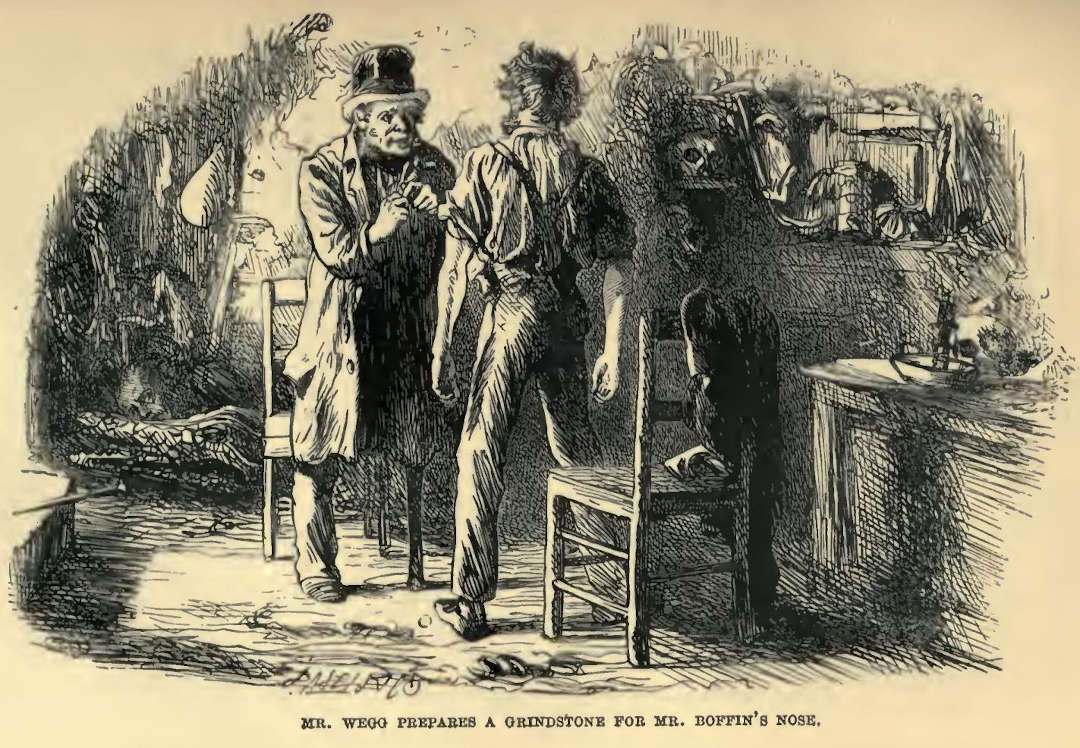
\includegraphics[scale=2.3]{03-14-01}

With this agreeable promise Wegg stumped out, and shut the shop-door
after him. ‘Wait till I light a candle, Mr Boffin,’ said Venus, ‘and
you’ll come out more comfortable.’ So, he lighting a candle and holding
it up at arm’s length, Mr Boffin disengaged himself from behind the
alligator’s smile, with an expression of countenance so very downcast
that it not only appeared as if the alligator had the whole of the joke
to himself, but further as if it had been conceived and executed at Mr
Boffin’s expense.

‘That’s a treacherous fellow,’ said Mr Boffin, dusting his arms and legs
as he came forth, the alligator having been but musty company. ‘That’s a
dreadful fellow.’

‘The alligator, sir?’ said Venus.

‘No, Venus, no. The Serpent.’

‘You’ll have the goodness to notice, Mr Boffin,’ remarked Venus, ‘that I
said nothing to him about my going out of the affair altogether, because
I didn’t wish to take you anyways by surprise. But I can’t be too soon
out of it for my satisfaction, Mr Boffin, and I now put it to you when
it will suit your views for me to retire?’

‘Thank’ee, Venus, thank’ee, Venus; but I don’t know what to say,’
returned Mr Boffin, ‘I don’t know what to do. He’ll drop down on me any
way. He seems fully determined to drop down; don’t he?’

Mr Venus opined that such was clearly his intention.

‘You might be a sort of protection for me, if you remained in it,’ said
Mr Boffin; ‘you might stand betwixt him and me, and take the edge off
him. Don’t you feel as if you could make a show of remaining in it,
Venus, till I had time to turn myself round?’

Venus naturally inquired how long Mr Boffin thought it might take him to
turn himself round?

‘I am sure I don’t know,’ was the answer, given quite at a loss.
‘Everything is so at sixes and sevens. If I had never come into the
property, I shouldn’t have minded. But being in it, it would be very
trying to be turned out; now, don’t you acknowledge that it would,
Venus?’

Mr Venus preferred, he said, to leave Mr Boffin to arrive at his own
conclusions on that delicate question.

‘I am sure I don’t know what to do,’ said Mr Boffin. ‘If I ask advice of
any one else, it’s only letting in another person to be bought out, and
then I shall be ruined that way, and might as well have given up the
property and gone slap to the workhouse. If I was to take advice of my
young man, Rokesmith, I should have to buy HIM out. Sooner or later, of
course, he’d drop down upon me, like Wegg. I was brought into the world
to be dropped down upon, it appears to me.’

Mr Venus listened to these lamentations in silence, while Mr Boffin
jogged to and fro, holding his pockets as if he had a pain in them.

‘After all, you haven’t said what you mean to do yourself, Venus. When
you do go out of it, how do you mean to go?’

Venus replied that as Wegg had found the document and handed it to him,
it was his intention to hand it back to Wegg, with the declaration that
he himself would have nothing to say to it, or do with it, and that Wegg
must act as he chose, and take the consequences.

‘And then he drops down with his whole weight upon ME!’ cried Mr Boffin,
ruefully. ‘I’d sooner be dropped upon by you than by him, or even by you
jintly, than by him alone!’

Mr Venus could only repeat that it was his fixed intention to betake
himself to the paths of science, and to walk in the same all the days
of his life; not dropping down upon his fellow-creatures until they were
deceased, and then only to articulate them to the best of his humble
ability.

‘How long could you be persuaded to keep up the appearance of remaining
in it?’ asked Mr Boffin, retiring on his other idea. ‘Could you be got
to do so, till the Mounds are gone?’

No. That would protract the mental uneasiness of Mr Venus too long, he
said.

‘Not if I was to show you reason now?’ demanded Mr Boffin; ‘not if I was
to show you good and sufficient reason?’

If by good and sufficient reason Mr Boffin meant honest and
unimpeachable reason, that might weigh with Mr Venus against his
personal wishes and convenience. But he must add that he saw no opening
to the possibility of such reason being shown him.

‘Come and see me, Venus,’ said Mr Boffin, ‘at my house.’

‘Is the reason there, sir?’ asked Mr Venus, with an incredulous smile
and blink.

‘It may be, or may not be,’ said Mr Boffin, ‘just as you view it. But
in the meantime don’t go out of the matter. Look here. Do this. Give me
your word that you won’t take any steps with Wegg, without my knowledge,
just as I have given you my word that I won’t without yours.’

‘Done, Mr Boffin!’ said Venus, after brief consideration.

‘Thank’ee, Venus, thank’ee, Venus! Done!’

‘When shall I come to see you, Mr Boffin.’

‘When you like. The sooner the better. I must be going now. Good-night,
Venus.’

‘Good-night, sir.’

‘And good-night to the rest of the present company,’ said Mr Boffin,
glancing round the shop. ‘They make a queer show, Venus, and I should
like to be better acquainted with them some day. Good-night, Venus,
good-night! Thankee, Venus, thankee, Venus!’ With that he jogged out
into the street, and jogged upon his homeward way.

‘Now, I wonder,’ he meditated as he went along, nursing his stick,
‘whether it can be, that Venus is setting himself to get the better of
Wegg? Whether it can be, that he means, when I have bought Wegg out, to
have me all to himself and to pick me clean to the bones!’

It was a cunning and suspicious idea, quite in the way of his school
of Misers, and he looked very cunning and suspicious as he went jogging
through the streets. More than once or twice, more than twice or thrice,
say half a dozen times, he took his stick from the arm on which he
nursed it, and hit a straight sharp rap at the air with its head.
Possibly the wooden countenance of Mr Silas Wegg was incorporeally
before him at those moments, for he hit with intense satisfaction.

He was within a few streets of his own house, when a little private
carriage, coming in the contrary direction, passed him, turned round,
and passed him again. It was a little carriage of eccentric movement,
for again he heard it stop behind him and turn round, and again he saw
it pass him. Then it stopped, and then went on, out of sight. But, not
far out of sight, for, when he came to the corner of his own street,
there it stood again.

There was a lady’s face at the window as he came up with this carriage,
and he was passing it when the lady softly called to him by his name.

‘I beg your pardon, Ma’am?’ said Mr Boffin, coming to a stop.

‘It is Mrs Lammle,’ said the lady.

Mr Boffin went up to the window, and hoped Mrs Lammle was well.

‘Not very well, dear Mr Boffin; I have fluttered myself by
being--perhaps foolishly--uneasy and anxious. I have been waiting for
you some time. Can I speak to you?’

Mr Boffin proposed that Mrs Lammle should drive on to his house, a few
hundred yards further.

‘I would rather not, Mr Boffin, unless you particularly wish it. I feel
the difficulty and delicacy of the matter so much that I would rather
avoid speaking to you at your own home. You must think this very
strange?’

Mr Boffin said no, but meant yes.

‘It is because I am so grateful for the good opinion of all my
friends, and am so touched by it, that I cannot bear to run the risk of
forfeiting it in any case, even in the cause of duty. I have asked my
husband (my dear Alfred, Mr Boffin) whether it is the cause of duty,
and he has most emphatically said Yes. I wish I had asked him sooner. It
would have spared me much distress.’

[‘Can this be more dropping down upon me!’ thought Mr Boffin, quite
bewildered.)

‘It was Alfred who sent me to you, Mr Boffin. Alfred said, “Don’t
come back, Sophronia, until you have seen Mr Boffin, and told him all.
Whatever he may think of it, he ought certainly to know it.” Would you
mind coming into the carriage?’

Mr Boffin answered, ‘Not at all,’ and took his seat at Mrs Lammle’s
side.

‘Drive slowly anywhere,’ Mrs Lammle called to her coachman, ‘and don’t
let the carriage rattle.’

‘It MUST be more dropping down, I think,’ said Mr Boffin to himself.
‘What next?’



